\chapter{BOLÜM DÖRT BÜYÜK BAŞLIK}
%
\lipsum[7]
Şekil-\ref{fig:featureextraction}'de verilmiştir.
  
 \begin{figure}[!htb]
    \centering
    \begin{tikzpicture}[
      level 1/.style={sibling distance=90mm},
      edge from parent/.style={->,draw}, node distance=2.3cm,
      >=latex]
    
    % root of the the initial tree, level 1
    \node[root] {Diyagram}
    % The first level, as children of the initial tree
      child {node[level 2,yshift=-25pt] (c1) {Öznitelikler1}}
      child {node[level 2,yshift=-25pt] (c2) {Öznitelikler1}};
    
    % The second level, relatively positioned nodes
    \begin{scope}[every node/.style={level 3}]
    % \node [below of = c1, xshift=15pt] (c11) {Setting shape};
    % \node [below of = c11] (c12) {Choosing color};
    % \node [below of = c12] (c13) {Adding shading};
    
    \node [below of = c2, xshift=10pt] (c21) {Alt-1};
    \node [below of = c21] (c22) {Alt-2};
    
    % \node [below of = c3, xshift=15pt] (c31) {Default arrows};
    % \node [below of = c31] (c32) {Arrow library};
    % \node [below of = c32] (c33) {Resizing tips};
    % \node [below of = c33] (c34) {Shortening};
    % \node [below of = c34] (c35) {Bending};
    \end{scope}
    
    % lines from each level 1 node to every one of its "children"
    % \foreach \value in {1,2,3}
    %   \draw[->] (c1.195) |- (c1\value.west);
    
    \foreach \value in {1,...,2}
      \draw[->] (c2.195) |- (c2\value.west);
    
    % \foreach \value in {1,...,5}
    %   \draw[->] (c3.195) |- (c3\value.west);
    \end{tikzpicture}
    \caption{Diyagram-1}
    \label{fig:featureextraction}
\end{figure}
% \lipsum[1-2]  


\section{Alt-1}

\lipsum[5] .~Algoritma~\ref{alg:psoudocode} 
\lipsum[8] Şekil-\ref{fig:geofeats}'de verilmiştir.

\begin{figure}[h]
\centering
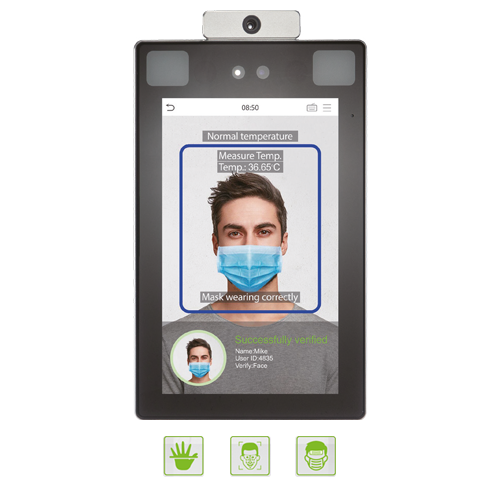
\includegraphics[trim={0.5cm 0.4cm 0.5cm 2cm},clip,width=0.80\textwidth]{gorseller/temp_image.png}
\caption{temp image}\label{fig:geofeats}
\end{figure}

\RestyleAlgo{ruled}

%% This is needed if you want to add comments in
%% your algorithm with \Comment
\SetKwComment{Comment}{/* }{ */}
\vspace{0cm}
\begin{algorithm}[htp]
\caption{x Algoirtması}\label{alg:psoudocode}
\KwData{$P$}
\KwResult{$y = [ ]$}
$y_{1} \gets [ ]$\;
$y_{2} \gets [ ]$\;
% $X \gets x$\;
$N \gets 1$\;
\While{$N \leq 68$}{
  \eIf{$N$ is even}{
    $y_{1} \gets dis(P(N),P(N+2))$\;
    $N \gets N + 1 $ \Comment*[r]{Bu aşama tekrarlanır.}
  }{\If{$N$ is odd}{
      $y_{2} \gets dis(P(N),P(N+2))$\;
      $N \gets N + 1 $ 
    }
  }
}
$y \gets y_{1} + y_{2} $
\end{algorithm}

% =========================

\newpage
\section{Alt Bölüm Birinci Derece}

\lipsum[8] \acrfull{lbp}, \acrfull{lmp}, \acrfull{ldp}, ve \acrfull{hog} 
\lipsum[6]
\acrshort{lbp}  \acrshort{hog} 
% =========================

\subsection{Alt Bölüm İkinci Derece}

\acrfull{hog}. 
\lipsum[12]. 
\acrshort{hog} 49 Şekil-\ref{flow:hog}'de gösterilmiştir. 

\begin{figure}[!htb]
    \centering
    \begin{tikzpicture}[
      >=latex',
      auto
    ]
    \node [intg] (ks)  {start};
      \node [intg] (kp) [node distance=1.8cm,below of=ks]  {nofe};
      \node [int]  (ki1) [node distance=1.5cm and -1cm,below left=of kp] {node};
      \node [int]  (ki2) [node distance=1.5cm and -1cm,below right=of kp] {node2};
      \node [intg] (hc1) [node distance=2cm,below of=ki1] {part1};
      \node [intg] (hc2) [node distance=2cm,below of=ki2] {part2};
      \node [intg] (ki3) [node distance=6.5cm,below of=kp] {share};
      \node [intg] (ki4) [node distance=2cm,below of=ki3] {final};

      \draw[->] (kp) -- ($(kp.south)+(0,-0.75)$) -| (ki1) node[above,pos=0.25] {} ;
      \draw[->] (kp) -- ($(kp.south)+(0,-0.75)$) -| (ki2) node[above,pos=0.25] {};
      \draw[->] (hc1) |- (ki3);
      \draw[->] (hc2) |- (ki3);
      \draw[->] (ki3) -- (ki4);
      \draw[->] (ks) -- (kp);
      \draw[->] (ki1) -- (hc1);
      \draw[->] (ki2) -- (hc2);
    \end{tikzpicture}
	\caption{flow chart}%\cite{paper12}.}
	\label{flow:hog}%
\end{figure}


\acrshort{hog} 
 \lipsum[12-14].

Önce $G_x$ ve $G_y$ hesaplanır. İlk $G_x$ ve $G_y$ değeri  Eşitlik-\ref{equ:hoggx}'deki formül kullanılarak hesaplanır. $r,c$ dir. $I$ asldır.

\begin{equation}
    \begin{aligned}
    G_{x}(r,c) = I(r,c+1) - I(r,c-1) 
    \\ 
    G_{y}(r,c) = I(r-1,c) - I(r+1,c) 
    \end{aligned}
 \label{equ:hoggx}
\end{equation}

$G_x$ ve $G_y$,  sonra Eşitlik-\ref{equ:hoggx2}'de sırtımsak.

\begin{equation}
    \begin{aligned}
    \textit{Büyüklük}(\mu) = \sqrt{G_{x}^{2}+G_{y}^{2}}
    \\ 
    \textit{Açı}(\theta) = \left| tan^{-1}(G_{y}/G_{x}) \right| 
    \end{aligned}
 \label{equ:hoggx2}
\end{equation}


% =========================

\newpage
\subsection{Alt Bölüm İkinci Derece2}


\lipsum[11-14]

Eşitlik-\ref{equ:lbpdistc}'de  $n$, - $t_1$, aralarındaki mesafe uzaklığı ise $d_n$ olarak gösterilmniştir.

\begin{equation}
  d_n = \sqrt{{(n_x - t_{1_x})^2}+{(n_y - t_{1_y})^2}}
 \label{equ:lbpdistc}
\end{equation}

\lipsum[5]

\begin{equation}
x = my+5 \begin{cases}
-R< i,j<R &\text{$i,j\in Z$}\\
{d_n}<R
\end{cases}
\label{equ:lbpcalc}
\end{equation}

\lipsum[6]



%\begin{equation}
\begin{equation}
    t = y^2 + x^3
    \label{eq:lbp}%
\end{equation}

\lipsum[16]

\begin{equation}
f = \sum_{i} l_{i} \begin{cases}
 0< i<68 &\text{$i\in Z$}
\end{cases}
\label{eq:4}%
\end{equation}

